% !TEX root = ../report.tex

\chapter{Electrical}\label{electrical}

\section{Power Distribution and Motor Drive}\label{elec/poweranddrive}
Overview of system and why we bought it
\subsection{Testing}\label{elec/poweranddrive/test}
motor drive system test circiut
should test power distribrutionat somepoint 


\section{Range Sensors}\label{elec/range}
For the robot to localise itself, it needs to be able to measure the distance between itself and the surrounding environment. By recording the measurements relative to the robots current position, a point map can be built up over time and a general map of the environment can be constructed. 

\subsection{Design}\label{elec/range/design}
Infra-red, ultrasound and LIDAR distance were all considered. These are all active sensors, meaning that they measure the effect of an output from the sensor, in these cases, IR light, ultrasonic waves or visible light respectively. 

Of these three, LIDAR is generally considered to be the most effective as it is the most accurate and has a \ang{360} field of view However, it is both too expensive and too heavy for our application, especially considering that each robot would need one. 
\todo{infra red}
Ultrasonic transceivers were therefore decided upon for use in this project. These work by transmitting sound at a particular frequency and measuring the time until the reflected wave returns to the sensor. These are also cheap, but produce a wider cone of transmission than the IR sensors, making them less likely to miss objects at the cost of accuracy in the direction of the measurement. 

The ultrasonic sensor used was the HC-SR04
\todo{merge with mech section}

other considerations +tives and -tives
Ultrasonic system theory
Sensor selected and why


%\begin{figure}[!ht]
%	\centering
%	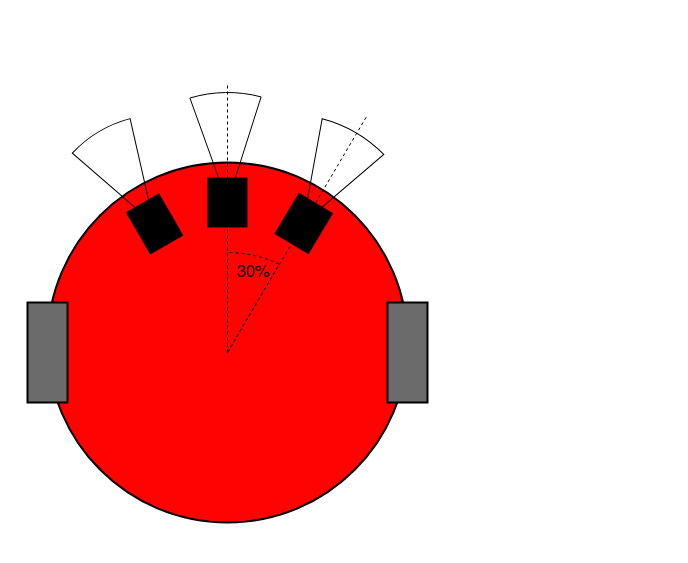
\includegraphics[width=0.5\textwidth]{UltraSoundSensorDiagram}
%	\caption{Ultrasound Sensor Layout}\label{UltraSoundSensorDiagram}

%\end{figure}

\subsection{Implementation}\label{elec/range/impl}
Sensor layout (3 deg cones) 
circuit layout
schematic

The hardware required for the ultrasonic sensors is relatively straight forwards. They are each connected to a 5V supply and ground, and the other two pins are connected to standard GPIO pins on the RPi. The echo pin has to be connected through a voltage divider as the RPi is only rated at 3.3V compared to the sensor's 5V. The trig pin can be connected directly to the RPi, however, as 3.3V is above the threshold voltage\todo{cite sensor DS}.

The distances are measured by an \textit{USScan} class. This has a \textit{get\_scan()} function which iterates through each ultrasonic sensor and takes a reading, as shown below in Code Listing \ref{lst:get_scan}

\begin{lstlisting}[caption={get\_scanFunction in USScan},label={lst:get_scan} , language=python]
def get_scan():
    """Get scan of ranges from all ultrasonic sensors.
    :return: (USScan) Scan of ranges
    :except: (UltrasonicTimeout) If module timed out waiting for GPIO input change
    """
    start = time.time()
    rl = get_range(LEFT)
    time_remaining = start + scan_increment - time.time()
    if time_remaining > 0:
        time.sleep(time_remaining)
    rc = get_range(CENTRE)
    time_remaining = start + 2 * scan_increment - time.time()
    if time_remaining > 0:
        time.sleep(time_remaining)
    rr = get_range(RIGHT)
    return USScan([rl, rc, rr])
\end{lstlisting}

This method allows the various readings to be taken without interfering with each other, as the second ultrasonic pulse isn't omitted until the first is received. 

As \ref{lst:get_scan} shows,\textit{get\_range()} is used by \textit{get\_scan()} to find the distance measured by each sensor. This simply triggers the sensor and times how long until the echo pin turns high. The range is then calculated by the equation $ 2d = tv_s$ where $v_s$ is the speed of sound. It is then converted to mm.

\subsection{Testing}\label{elec/range/test}
The sensors were initially tested using a signal generator and an oscilloscope. This allowed us to quickly identify 2 malfunctioning sensors, as there was a linear response between the distance to an obstacle and the width of the echo pin pulse width. The pulse width could then be used to to calculate the measured distance and this compared to the distance found with a measuring tape. Gave readings accurate to within a cm, however this method  was not repeated enough for any rigorous analysis of accuracy as the distance calculations would have to be performed manually and this was time consuming. 
\todo{images of testing waveform and maybe test cicuit schematic}

A circuit was then created to read the values using an Arduino microcontroller to allow the distance readings to be found quickly and the accuracy of the sensors measured.

\todo{rpi testing roomba node}




\section{Encoders}\label{elec/encoder}
Wheel encoders are required to measure the speed of each wheel independently. This gives the system far more control over its path as well as allowing it to perform dead reckoning through wheel odometry. 
\subsection{Design}\label{elec/encoder/design}
 The motors selected had both incremental and absolute custom designed encoder, but as only the wheel speed is needed and not the position, the incremental rotary encoders were used. These were hall effect encoders, which measure the changing magnetic field of magnets which are attached to the motor shaft. It has two 6 pole magnets magnets which create 12 counts per revolution of the motor shaft, which, after scaling for the gear ratio of 120:1, results in 1440 counts per revolution of the robot wheel. 
 
The encoders are quadrature encoders, which represent the speed and direction of the wheels with two square waves where the frequency represents the speed and which of the two waves is leading shows the direction.

\subsection{Implementation}\label{elec/encoder/impl}

The encoder data was read into the RPi by an encoder class written in Python. This worked by connecting call back methods to both the A and B channel pins. How this is initialised is shown in Code Listing \ref{lst:enc_event_detect}

\todo{format listings}

\begin{lstlisting}[caption={encoder callback set-up},label={lst:enc_event_detect} , language=python]
GPIO.add_event_detect(self.pin$_$a, GPIO.BOTH, callback=self._callback_a)
\end{lstlisting}

This then either increments or decrements a count depending on the direction, as shown in Code Listing \ref{lst:enc_callback}. Note that \textit{\_callback\_b()} is identical but with \textit{self.\_inc()} and \textit{self.\_dec()} switched.

\begin{lstlisting}[caption={Encoder Callback Function},label={lst:enc_callback} , language=python]
def _callback_a(self, _):
        a, b = GPIO.input(self.pin_a), GPIO.input(self.pin_b)
        if a == b:
            self._inc()
        else:
            self._dec()
\end{lstlisting}


\subsection{Testing}\label{elec/encoder/test}
The encoders were first tested to ensure that they functioned correctly using a test circuit and connecting the encoder outputs to an oscilloscope. All the encoders were shown to function correctly outputting square waves in both channels and with channel A leading B when the motor was moving forwards and B leading A when going forwards. \todo{check order}
\todo{get graph of output} 

\todo{system testing }

\section{IMU}\label{elec/imu}
The IMU consists of a three axis accelerometer and a three axis gyroscope which can be used to measure both the linear acceleration and rotational velocity of the robot. This can be integrated and double integrated to track the robots position over time again performing dead reckoning. The system can then perform sensor fusion on this data and the encoder readings to get far more accurate results than possible with either system independently. 


\subsection{Design}\label{elec/imu/design}
The IMU selected was the MPU-6050. It was the most accurate sensor of a similar budget with regards to noise, cross axis sensitivity and non linearity. Offset tolerance was also considered but this was less of a consideration as this can be compensated for as long as the offset is not so extreame as to limit the range. It was configured to operate in its smallest range of values ($\pm\ang{250}s^{-1}$ and $\pm2g$\cite{}\todo{citation}).

The IMU was to be placed as close to the centre of the axis of the robot as possible, as when it is far from the centre of rotation the centripetal forces acting on it can interfere and be measured as linear motion away from the centre.  

\subsection{Implementation}\label{elec/imu/impl}

The IMU selected uses the I$^2$C protocol for data transmission, which integrates well with the RPi as it has dedicated I$^2$C GPIO pins and existing libraries to facilitate communication. 

It should be noted that, while this was the only I$^2$C device currently used, other devices with conflicting addresses can be handled as The IMU allows the address to be changed through a data pin from 0x68 to 0x69. This would most likely be used if the framework developed was being used on another, more complicated system requiring several IMUs. This pin was not connected to the RPi in this design as it was not yet required. 
\todo{code description}

An \verb|i2c_object| class that used the smbus package was created to simplify the communication over the I\textsuperscript{2}C buses. These were initialised with an I\textsuperscript{2}C bus and an address, and contained various methods for reading and writing to the I\textsuperscript{2}C device. 

\todo{what code is interesting}

An \verb|IMU| class was then created to read the data from the IMU which and an \verb|i2c_object| instance. Code Listing \ref{lst:imu_init} shows the constructor for the IMU class. Note that the \verb|write_byte()| call is essential to enable the IMU transmissions. 

\begin{lstlisting}[caption={IMU Initialisation Function},label={lst:imu_init} , language=python]
def __init__(self, address, rate, channel=1):
    self.address = address
    self.IMU_i2c = i2c.i2c_object(self.address, channel=channel)
    self.rate = rate
    self.IMU_i2c.write_byte(0x6B, 0x00) # turns imu on
    self.speed_vect = (0.0, 0.0, 0.0)
\end{lstlisting}

As the IMU returns arbitrary values between -32768 and 32767 \todo{source}, a constant was required to convert the results to meaningful values. The calculations for these is shown in Code Listing \ref{lst:imu_units}. 

\begin{lstlisting}[caption={Calculation for IMU Value to SI unit Conversion Constants},label={lst:imu_units} , language=python]
GYRO_RANGE = 250  # deg/sec
GYRO_DIVISIONS = 32768  # 2 ^15
GYRO_UNITS = (GYRO_RANGE * math.pi * 2.0) / (GYRO_DIVISIONS * 360)  # rad/sec

ACC_RANGE = 2 * 9.81  # m/s^2
ACC_DIVISIONS = 32768  # 2 ^15
ACC_UNITS = ACC_RANGE / ACC_DIVISIONS  # m/s^2
\end{lstlisting}

The acceleration values can then be multiplied by the \textit{ACC\_UNITS} constant and the result is the acceleration in $ms^{-2}$, and \textit{GYRO\_UNITS} can be used similarly to find the rotation in $rads^{-1}$, as is shown in Code Listing \ref{lst:read_funcs}. 


\begin{lstlisting}[caption={Reading and Converting Raw IMU Values},label={lst:read_funcs} , language=python]
    def _read_gyro(self):
        x_rot_v = self.IMU_i2c.read_signed_word(0x43) * GYRO_UNITS
		...
        return (x_rot_v, y_rot_v, z_rot_v)

    def _read_accel(self):
        x_a = self.IMU_i2c.read_signed_word(0x3b) * ACC_UNITS
		...
        return (x_a, y_a, z_a)
\end{lstlisting}

The final step in reading the IMU results is to integrate the acceleration data as to get the linear velocities. This makes use of the \textit{speed\_vect} variable declared in the IMU constructor shown in Code Listing \ref{lst:imu_init}. \textit{speed\_vect} is incremented by the acceleration multiplied by the IMU rate, as shown in \ref{lst:imu_integration}.

\begin{lstlisting}[caption={Integrating Linear Acceleration},label={lst:imu_integration} , language=python]

def get_speeds(self):
		...
        accel_vect = self._read_accel()
        speed_vect = tuple([(1.0/self.rate) * accel_vect[i] + speed_vect[i] for i in range(len(accel_vect))])
        return speed_vect, gyro_speeds
\end{lstlisting}


\subsection{Testing}\label{elec/imu/test}
Initial work was performed with the IMU and an Arduino microcontroller before the RPis were acquired. The IMU was connected up and various movements were recorded. Python code was then written to interpret and visualise the data as a moving frame. 

\section{PCB}\label{elec/pcb}
As precise and consistent placement of components was required to ensure homogeneity of the robots, it was decided to develop a PCB for the connection and mounting of the parts (as opposed to using strip board).  
\subsection{Design}\label{elec/pcb/design}
The PCB required to contain the following components:
\begin{itemize}
  \item Raspberry Pi ribbon cable connector
  \item Three ultrasonic sensors
  \item IMU
  \item Left and right encoder connectors
  \item Motor drive connectors
  \item Power connectors
  \item LEDs for debugging
\end{itemize}

with the following design constraints:

\begin{itemize}
  \item Central ultrasonic sensor at the centre of the robot in the x axis
  \item the other ultrasonic sensors symmetrical about the y axis
  \item IMU chip in centre of axis
  \item Mounting holes for RPi and for mounting PCB to chassis
  \item Power connectors at fixed position relative to centre to ensure it connects to header on power distribution board
  \item Motor drive connectors also at fixed position relative to centre 
\end{itemize}
\todo{maybe find coordinates of parts for fixed position components}
With these constraints the following PCB design shown in figure \todo{image and reference}

Note that the peculiar shape is to allow room for the motors and encoders. 

\subsection{Testing}\label{elec/pcb/test}

After the components were soldered into place on the PCB, manual continuity tests were performed with a multimeter to ensure that adjacent pins had not been connected in the soldering process.

The PCB was then mounted and each module test was rerun to ensure that the connections were all correct. This process exposed a flaw as one of the ultrasonic sensors seemed to no longer work. After some investigation it was noticed that the screws being used had slightly larger heads than the screws used for mounting the test strip board and was connecting two tracks. A rubber washer was used as temporary fix and then this was corrected in the final PCB design. 
